\section{Desarrollo: Caso 1, configuración VFA-VFA}
\label{sec:desarrollo_c1}

\subsection{Diseño}
\label{sec:diseno_c1}

Partiendo de las características del amplificador LM324 (\autoref{tab:param_vfa}) se dimensionaron las resistencias $R_i$, $R_f$, $R_1$ y $R_2$. El segundo amplificador ($A_{02}$) está dentro del lazo global, por lo que la ganancia a lazo cerrado queda fijada por la red $R_i$--$R_f$ (\autoref{eq:ganancia_LC_NI_2}). La máxima planicidad de módulo ($Q_p = 0{,}707$) se logra compensando por desplazamiento de polos con la red local $R_1$--$R_2$ de $A_{02}$, para lo cual la ganancia de la segunda etapa debe ser $A_{vf2} = Q_p\sqrt{A_{vf}}$ (\autoref{eq:Avf2_MPM}).

Los cálculos se automatizaron en un cuaderno de Jupyter (Caso 1). En la \autoref{tab:parametros_vfa_vfa} se reúnen las expresiones utilizadas, su evaluación numérica y el valor resultante de cada parámetro de diseño, junto con la verificación de la condición de MPM ($D_p = 2T_0$, \autoref{eq:Dp_MPM}).

\begin{table}[H]
\centering
\caption{Diseño VFA-VFA con $Q_p = 0{,}707$: expresiones, cálculo y valores.}
\label{tab:parametros_vfa_vfa}
\footnotesize
\setlength{\tabcolsep}{4pt}
\begin{tabular}{>{\raggedright\arraybackslash}p{0.31\textwidth} >{\centering\arraybackslash}p{0.2\textwidth} >{\centering\arraybackslash}p{0.27\textwidth} >{\centering\arraybackslash}p{0.13\textwidth}}
\toprule
\textbf{Parámetro} & \textbf{Expresión} & \textbf{Cálculo} & \textbf{Valor} \\
\midrule
Ganancia a lazo cerrado global $A_{vf}$ & dato & \SI{20}{dB} $\rightarrow 10^{20/20}$ & \SI{10}{V/V} \\
Factor de realimentación $K$ & $1/A_{vf}$ & $1/10$ & \num{0,1} \\
Resistencia de entrada global $R_i$ & elegida & --- & \SI{10}{k\ohm} \\
Resistencia de realimentación global $R_f$ & $R_i\,(A_{vf}-1)$ & $10\text{ k}\Omega \cdot 9$ & \SI{90}{k\ohm} \\
Ganancia del segundo amplificador $A_{vf2}$ & $Q_p\sqrt{A_{vf}}$ & $0{,}707\cdot\sqrt{10}$ & \SI{2,236}{V/V} \\
Resistencia de entrada local $R_1$ & elegida & --- & \SI{10}{k\ohm} \\
Resistencia de realimentación local $R_2$ & $R_1\,(A_{vf2}-1)$ & $10\text{ k}\Omega\cdot 1{,}236$ & \SI{12,361}{k\ohm} \\
Frecuencia del polo desplazado $f_{px}$ & $f_T/A_{vf2}$ & $1\text{ MHz}/2{,}236$ & \SI{447,2}{kHz} \\
Ganancia de lazo en continua $T_0$ & $K\,A_{d0}\,A_{vf2}$ & $0{,}1\cdot 10^5 \cdot 2{,}236$ & \num{22361} (\SI{87,0}{dB}) \\
Separación de polos $D_p$ & $A_{d0}/A_{vf2}$ & $10^5/2{,}236$ & \num{44721} ($=2T_0$) \\
\bottomrule
\end{tabular}
\end{table}

\subsection{Resultados analíticos}
\label{sec:analitico_c1}

Con los valores de diseño de la \autoref{tab:parametros_vfa_vfa} ($T_0 = 22\,361$, $D_p = 2T_0$), y a partir de las \autoref{eq:wp_A}, \autoref{eq:omegaG}, \autoref{eq:wH_wp} y \autoref{eq:wGc} se obtienen los valores de la \autoref{tab:analitica_c1}.

\begin{table}[H]
\centering
\caption{Resultados analíticos (modelo de dos polos).}
\label{tab:analitica_c1}
\small
\setlength{\tabcolsep}{4pt}
\begin{tabular}{>{\raggedright\arraybackslash}p{0.37\textwidth} >{\centering\arraybackslash}p{0.31\textwidth} >{\centering\arraybackslash}p{0.2\textwidth}}
\toprule
\textbf{Magnitud} & \textbf{Expresión} & \textbf{Valor} \\
\midrule
Ancho de banda potencial $f_G$ & $f_T/\sqrt{A_{vf}}$ & \SI{316,2}{kHz} \\
Cruce de $T$ compensada (asintótico) $f_{Gc}$ & $K\,A_{vf2}\,f_T$ & \SI{223,6}{kHz} \\
Cruce de $T$ compensada (exacto) & $|T(jf)|=1$ & \SI{203,5}{kHz} \\
Cruce de $T$ compensada respecto de $f_p$, $\Omega_G = f_{Gc}/f_p$ & \autoref{eq:omegaG} & \num{0,644} \\
Margen de fase $M_\varphi$ & \autoref{eq:Mphi_2polos} y \autoref{eq:Mphi_MPM} & \ang{65,53} \\
Frecuencia de los polos $f_p$ & \autoref{eq:wp_A} & \SI{316,2}{kHz} \\
Factor de calidad $Q_p = 1/(2\zeta)$ & \autoref{eq:wp_A} & \num{0,707} \\
Polo de lazo cerrado & $s_{1,2}$ & $(-223{,}6 \pm j\,223{,}6)$ kHz \\
Ancho de banda real $f_H$ ($-3$ dB) & \autoref{eq:wH_wp} & \SI{316,2}{kHz} \\
\bottomrule
\end{tabular}
\end{table}

Como se explicó en la \autoref{sec:bw}, el ancho de banda real coincide con el potencial ($f_H = f_G$), mientras que la frecuencia $f_{Gc}$ en la que cruza la ganancia de lazo compensada es menor y es la que se observa en la simulación del lazo.

Dado que el LM324 real tiene un segundo polo en $f_2 = 5{,}06\text{ MHz}$, se evaluó también un modelo de cuatro polos (dos polos $f_1$ y dos $f_2$ en el lazo abierto del compuesto, con la etapa compensada incluida), cuyos resultados se muestran en la \autoref{tab:modelos_c1}.

\begin{table}[H]
\centering
\caption{Resultados numéricos: modelo de 2 polos y de 4 polos.}
\label{tab:modelos_c1}
\begin{tabular}{lcc}
\toprule
\textbf{Magnitud} & \textbf{2 polos} & \textbf{4 polos} \\
\midrule
Frecuencia crítica $f_{Gc}$ [kHz] & 203,5 & 206,1 \\
Margen de fase [$^\circ$] & 65,53 & 62,51 \\
Margen de ganancia [dB] & $\infty$ & 21,4 \\
Ancho de banda real ($-3$ dB) [kHz] & 316,2 & 345,8 \\
Frecuencia de los polos $f_p$ [kHz] & 316,2 & 330,3 \\
Factor de calidad $Q_p$ & 0,707 & 0,746 \\
Polos dominantes [kHz] & $-223{,}6 \pm j\,223{,}6$ & $-221{,}4 \pm j\,245{,}1$ \\
\bottomrule
\end{tabular}
\end{table}

\emph{Nota:} el margen de ganancia del modelo de dos polos es infinito porque la fase de $T(s)$ tiende asintóticamente a $-180^\circ$ sin alcanzarlo a ninguna frecuencia finita; con cuatro polos la fase sí cruza $-180^\circ$ y el margen de ganancia es finito.

\begin{figure}[H]
    \centering
    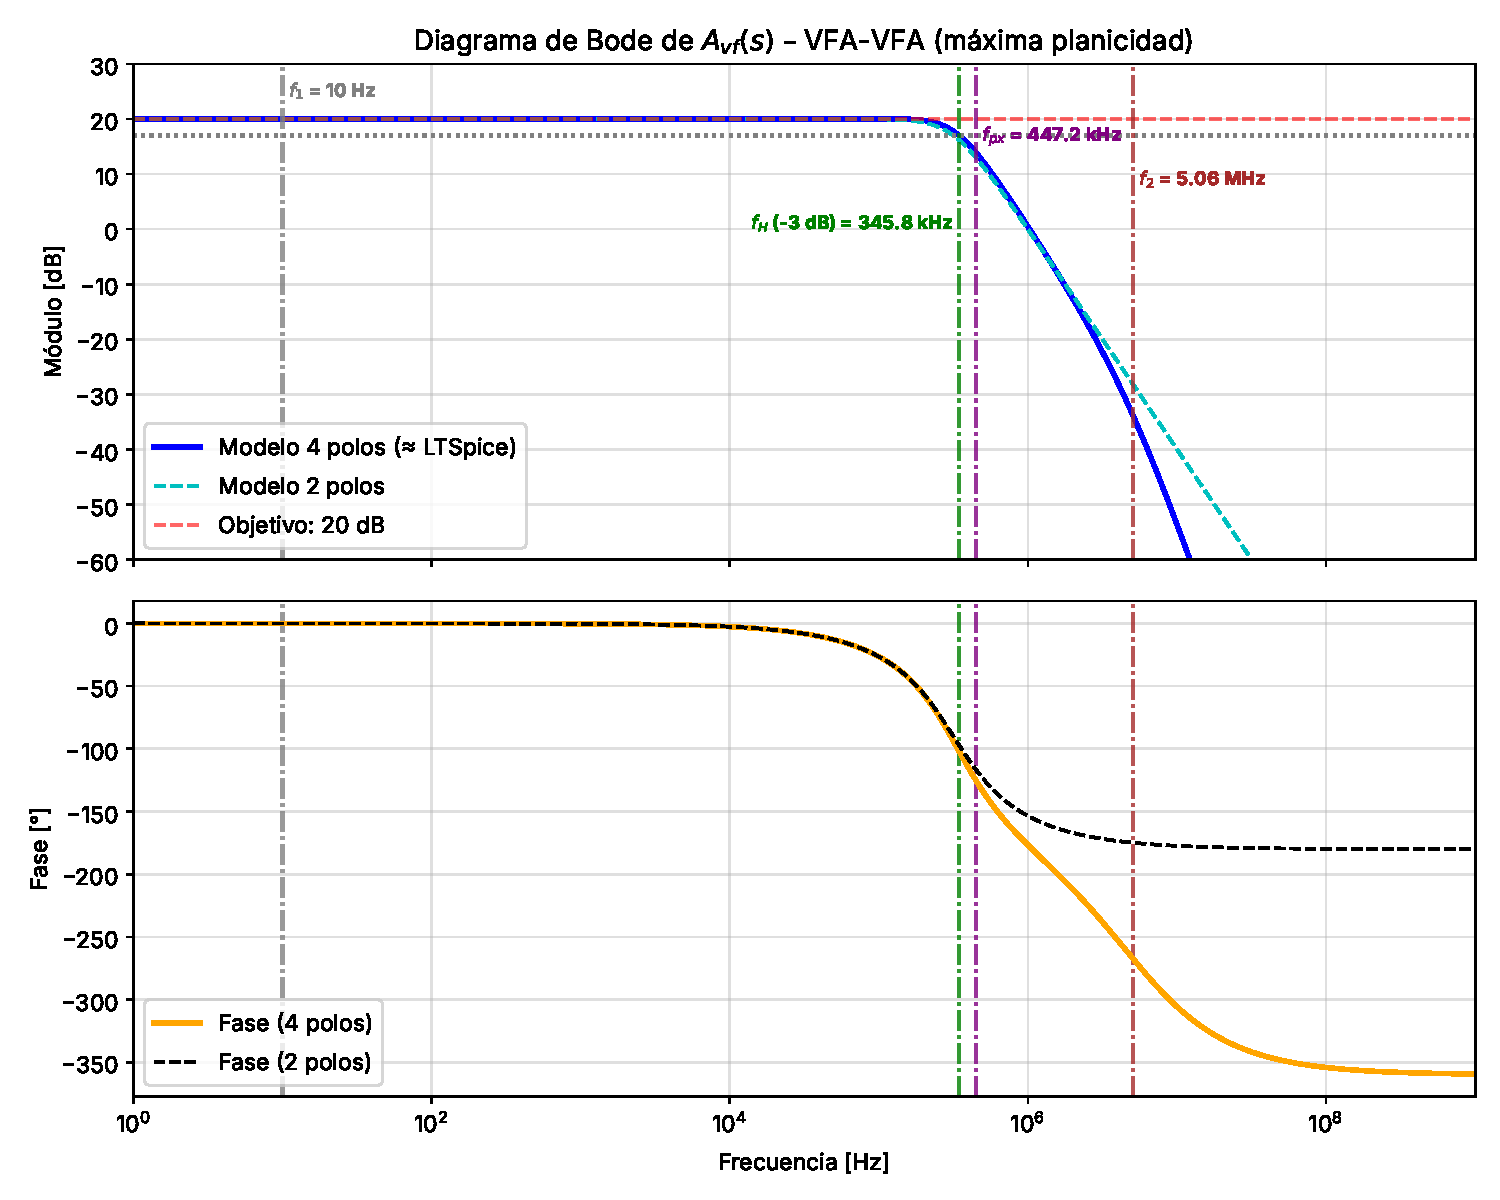
\includegraphics[width=0.95\linewidth,height=0.42\textheight,keepaspectratio]{Imagenes/c1_bode_lazo_cerrado.pdf}
    \caption{Diagrama de Bode a lazo cerrado (modelos de 2 y 4 polos). Se observa la ausencia de sobrepico, propia de MPM.}
    \label{fig:bode_lc_c1}
\end{figure}

\begin{figure}[H]
    \centering
    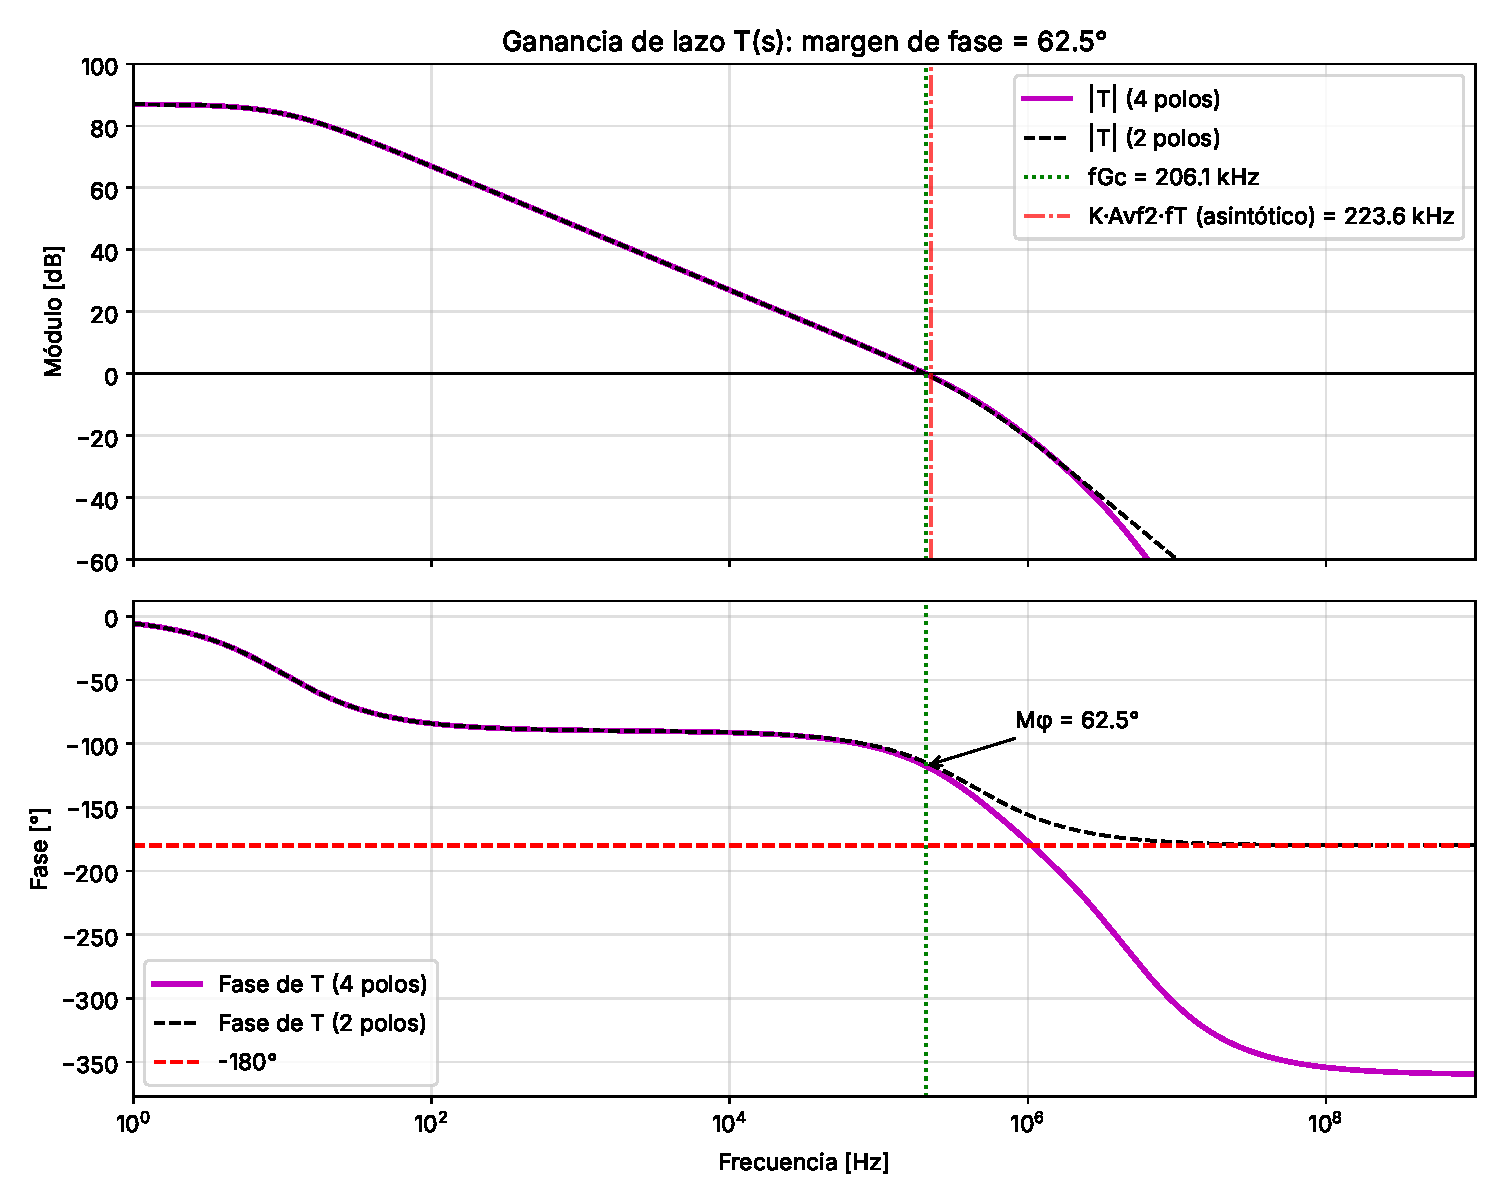
\includegraphics[width=0.95\linewidth,height=0.42\textheight,keepaspectratio]{Imagenes/c1_bode_ganancia_lazo.pdf}
    \caption{Diagrama de Bode de la ganancia de lazo: frecuencia crítica y margen de fase.}
    \label{fig:bode_lazo_c1}
\end{figure}

\paragraph{Respuesta al escalón teórica.} La \autoref{fig:escalon_teorico_c1} muestra la respuesta a un escalón de $0{,}1\text{ V}$ (salida de $1\text{ V}$) de los modelos de dos y de cuatro polos; los sobrepicos y el margen de fase estimado se comparan con la simulación en la \autoref{tab:escalon_c1}.

\begin{figure}[H]
    \centering
    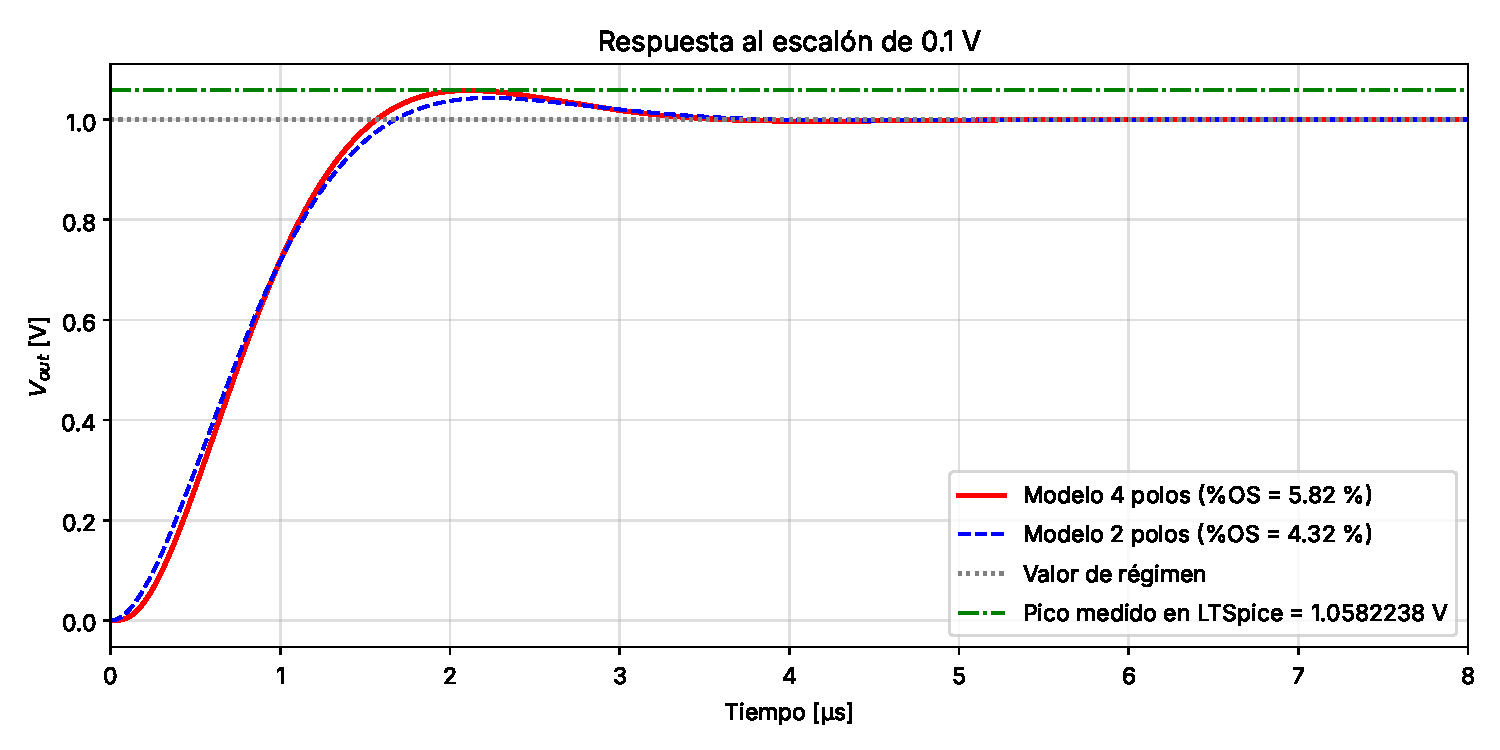
\includegraphics[width=0.95\linewidth,height=0.42\textheight,keepaspectratio]{Imagenes/c1_escalon_teorico.pdf}
    \caption{Respuesta al escalón teórica (2 y 4 polos).}
    \label{fig:escalon_teorico_c1}
\end{figure}

\subsection{Simulación}
\label{sec:simulacion_c1}

Se simularon en LTSpice los circuitos de la \autoref{fig:circuito_VFA_VFA}: lazo abierto, ganancia de lazo y lazo cerrado, con el modelo del LM324 de la bibliografía. En el esquemático la red global se implementó con $R_i = 1\text{ k}\Omega$ y $R_f = 9\text{ k}\Omega$ (misma relación que en el diseño), y la local con $R_1 = 10\text{ k}\Omega$ y $R_2 = 12{,}361\text{ k}\Omega$.

\begin{figure}[H]
    \centering
    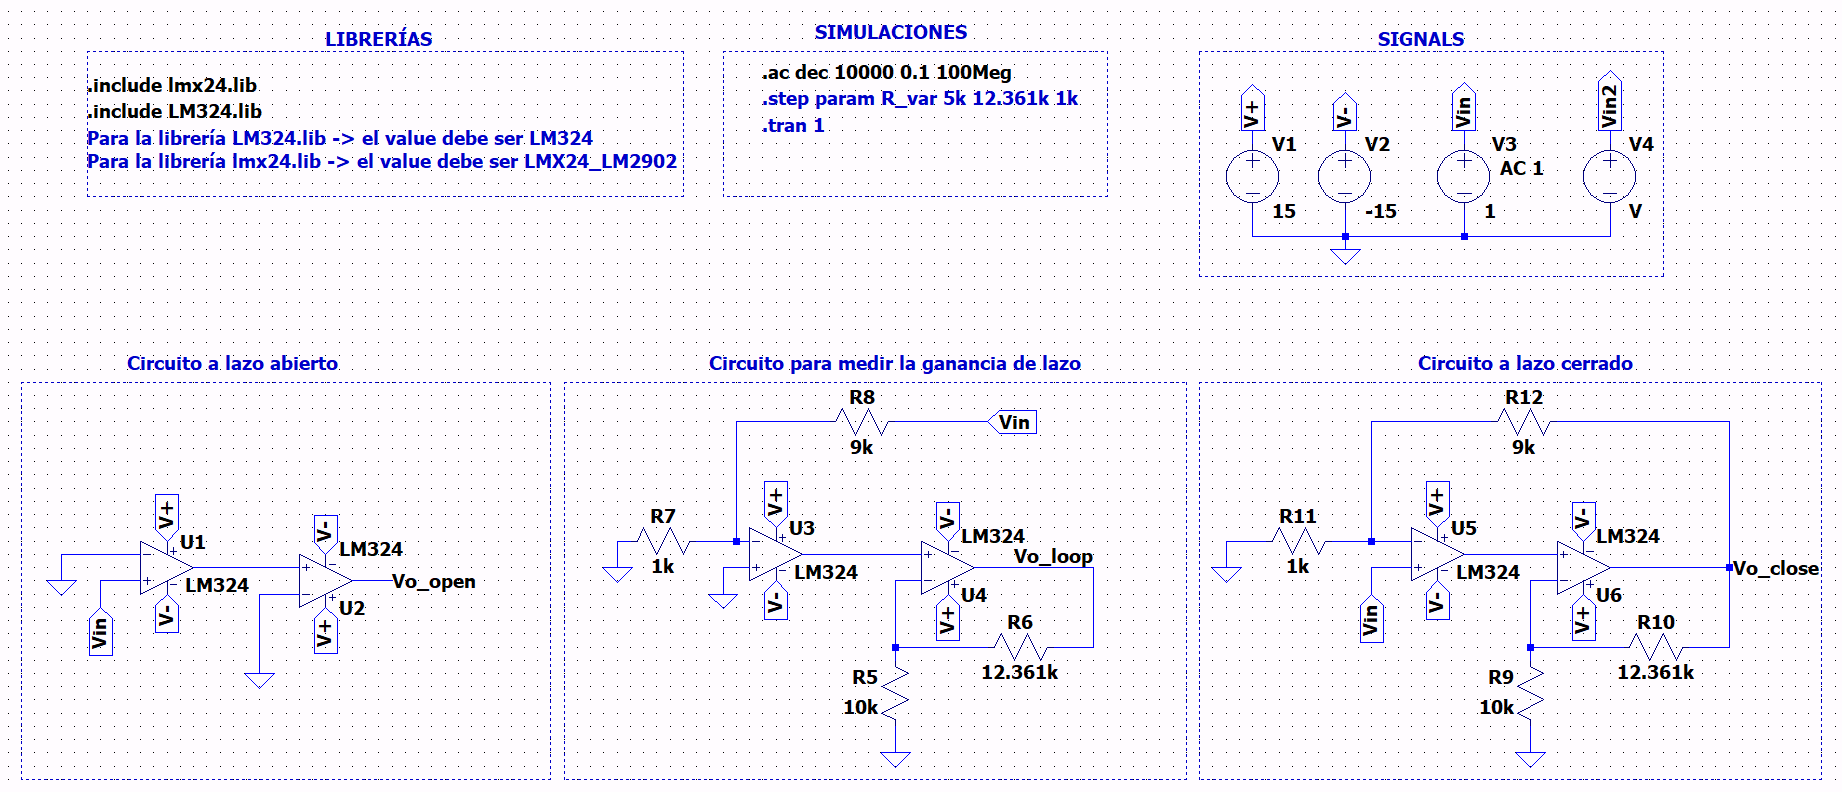
\includegraphics[width=\linewidth,height=0.32\textheight,keepaspectratio]{Imagenes/simulation_circuits_comp.png}
    \caption{Esquemático VFA-VFA, LTSpice.}
    \label{fig:circuito_VFA_VFA}
\end{figure}

\subsubsection{Respuesta en frecuencia a lazo abierto}
La \autoref{fig:rta_frec_open_loop_comp} muestra la respuesta a lazo abierto. Al tratarse de dos amplificadores idénticos en cascada, la ganancia en banda media es $A_{d0}^2$ ($200\text{ dB}$) y los polos son dobles, en $f_1 = 10\text{ Hz}$ y $f_2 = 5{,}06\text{ MHz}$.

\begin{figure}[H]
    \centering
    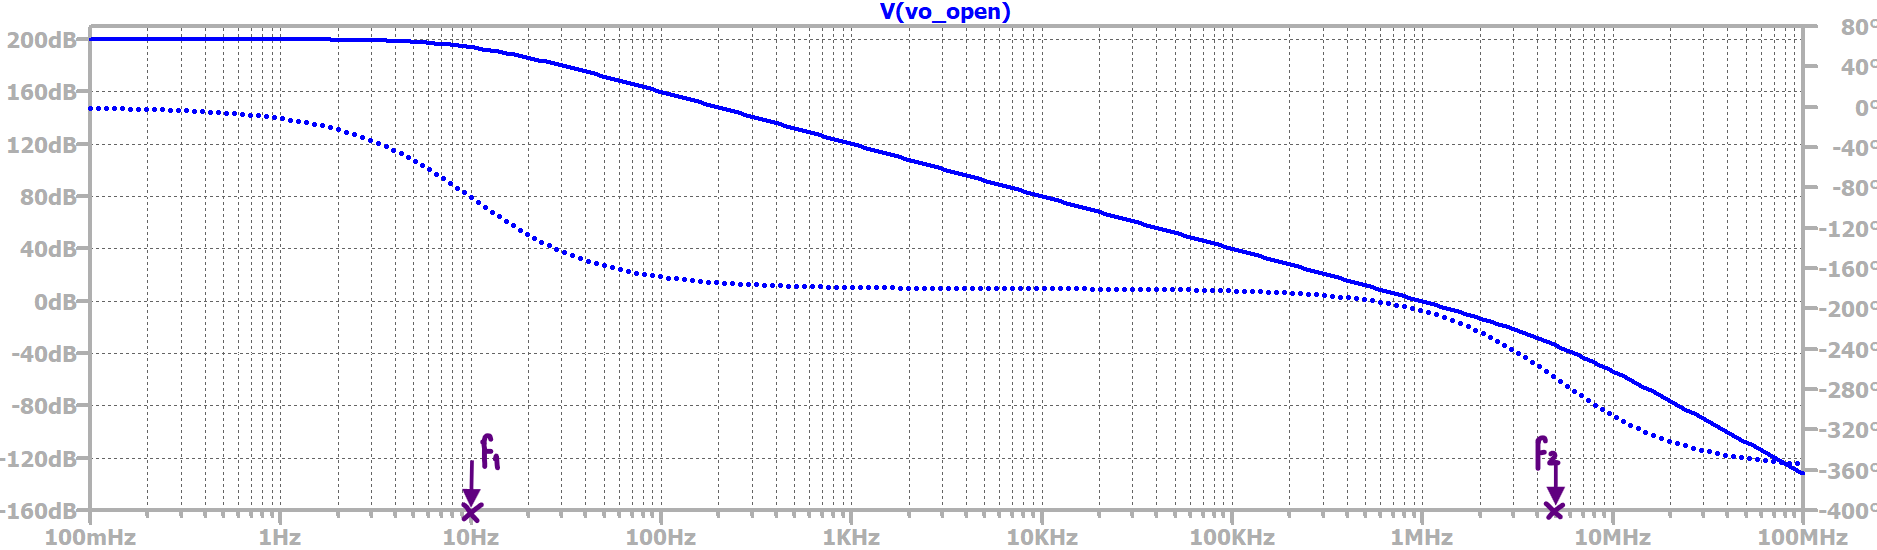
\includegraphics[width=\linewidth,height=0.32\textheight,keepaspectratio]{Imagenes/rta_frec_open_loop_comp.png}
    \caption{Respuesta en frecuencia a \textbf{lazo abierto}.}
    \label{fig:rta_frec_open_loop_comp}
\end{figure}

\subsubsection{Respuesta en frecuencia de la ganancia de lazo}
En la \autoref{fig:rta_frec_loop_comp.png} se midió con los cursores el punto de cruce de la ganancia de lazo, obteniéndose una frecuencia crítica $f_g \approx 206\text{ kHz}$ y un margen de fase $M_\varphi \approx 62{,}52^\circ$.

\begin{figure}[H]
    \centering
    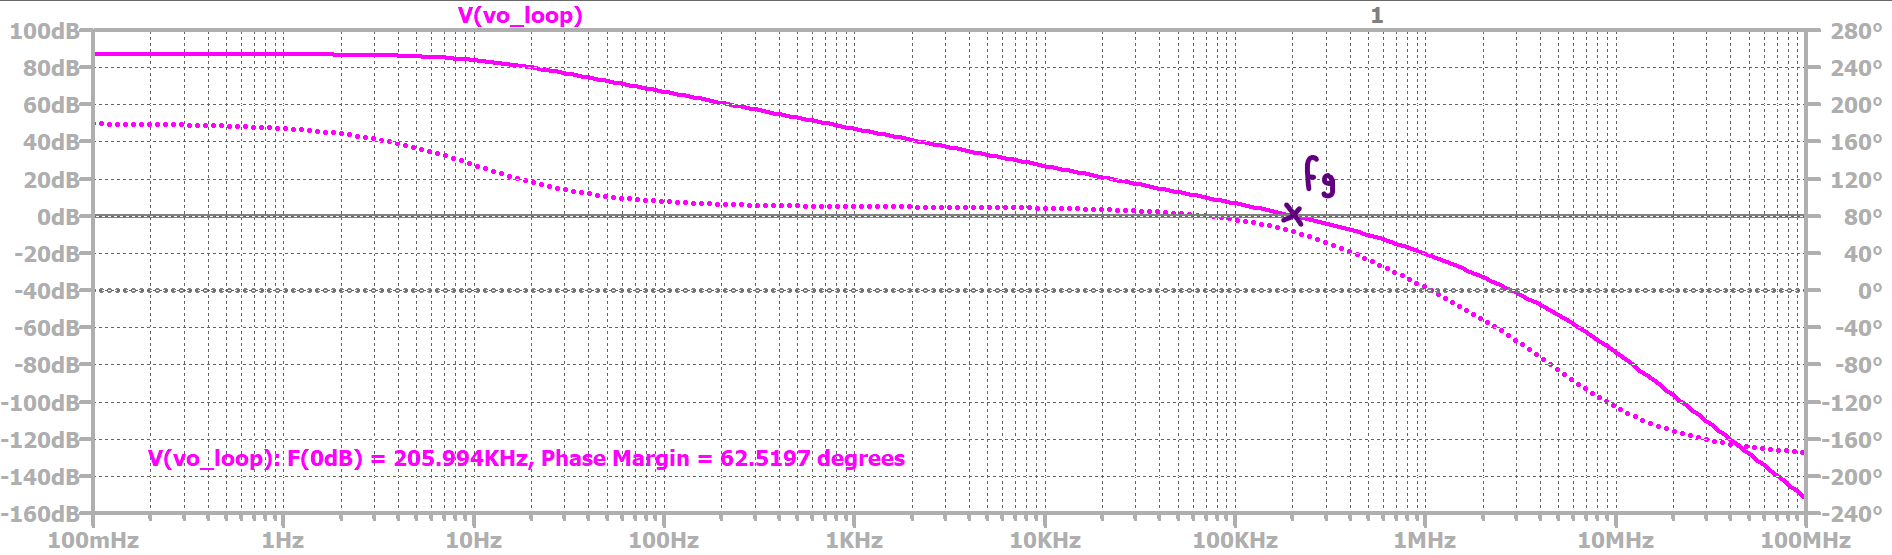
\includegraphics[width=\linewidth,height=0.32\textheight,keepaspectratio]{Imagenes/rta_frec_loop_comp.png}
    \caption{Respuesta en frecuencia de la \textbf{ganancia de lazo}.}
    \label{fig:rta_frec_loop_comp.png}
\end{figure}

\subsubsection{Respuesta en frecuencia a lazo cerrado}
La \autoref{fig:rta_frec_close_loop_BW_comp} confirma la ganancia en banda media de $20\text{ dB}$. El ancho de banda real medido, donde la ganancia cae $3\text{ dB}$ (a $17\text{ dB}$), es $f_H = 345\text{ kHz}$. La caída suave, sin sobrepico, valida la compensación por desplazamiento de polos.

\begin{figure}[H]
    \centering
    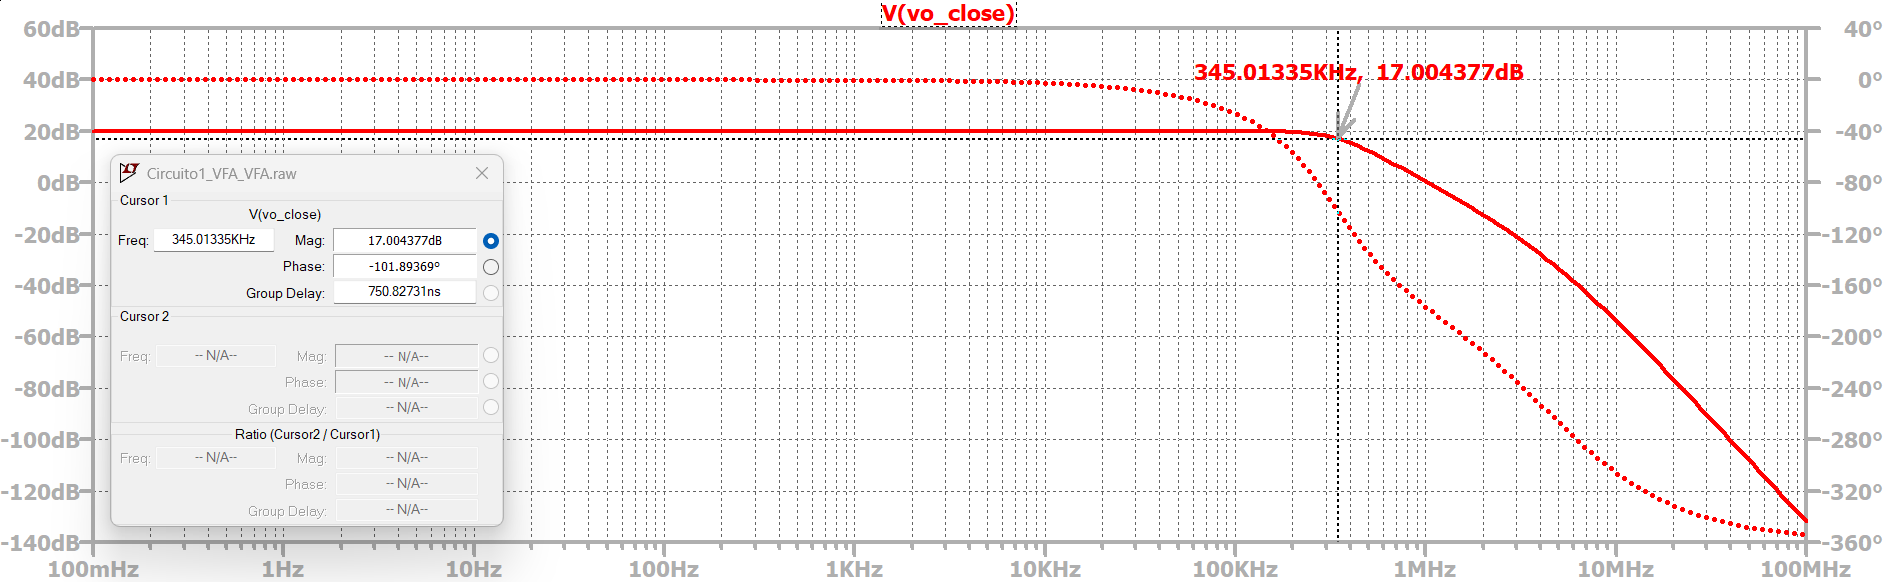
\includegraphics[width=\linewidth,height=0.32\textheight,keepaspectratio]{Imagenes/rta_frec_close_loop_BW_comp.png}
    \caption{Respuesta en frecuencia a \textbf{lazo cerrado}.}
    \label{fig:rta_frec_close_loop_BW_comp}
\end{figure}

\subsubsection{Respuesta al escalón}
Se aplicó un escalón de $0{,}1\text{ V}$ (salida de $1\text{ V}$), con tiempos de subida y de bajada de $10\text{ ns}$ y un paso máximo de simulación de $5\text{ ns}$. El flanco es mucho más rápido que el tiempo de subida del circuito ($\approx 1\,\mu\text{s}$), de modo que el sobrepico depende solo del circuito, y la amplitud pequeña evita que el \emph{slew rate} limite la respuesta. Se midieron $V_{pico} = 1{,}0582\text{ V}$ y $V_{estacionario} = 0{,}99995\text{ V}$. Aplicando las \autoref{eq:OS}, \autoref{eq:zeta} y \autoref{eq:MF_exacta} (\autoref{sec:escalon_mf}):
\begin{equation}
    \mathrm{\char37}OS = \frac{1{,}0582 - 0{,}99995}{0{,}99995}\cdot 100 = 5{,}83\,\mathrm{\char37}
\end{equation}
\begin{equation}
    \zeta = \frac{-\ln(0{,}0583)}{\sqrt{\pi^2 + \ln^2(0{,}0583)}} \approx 0{,}671
\end{equation}
\begin{equation}
    MF = \arctan\left( \frac{2\cdot 0{,}671}{\sqrt{\sqrt{1+4(0{,}671)^4}-2(0{,}671)^2}} \right) \approx 63{,}6^\circ
\end{equation}

\begin{figure}[H]
    \centering
    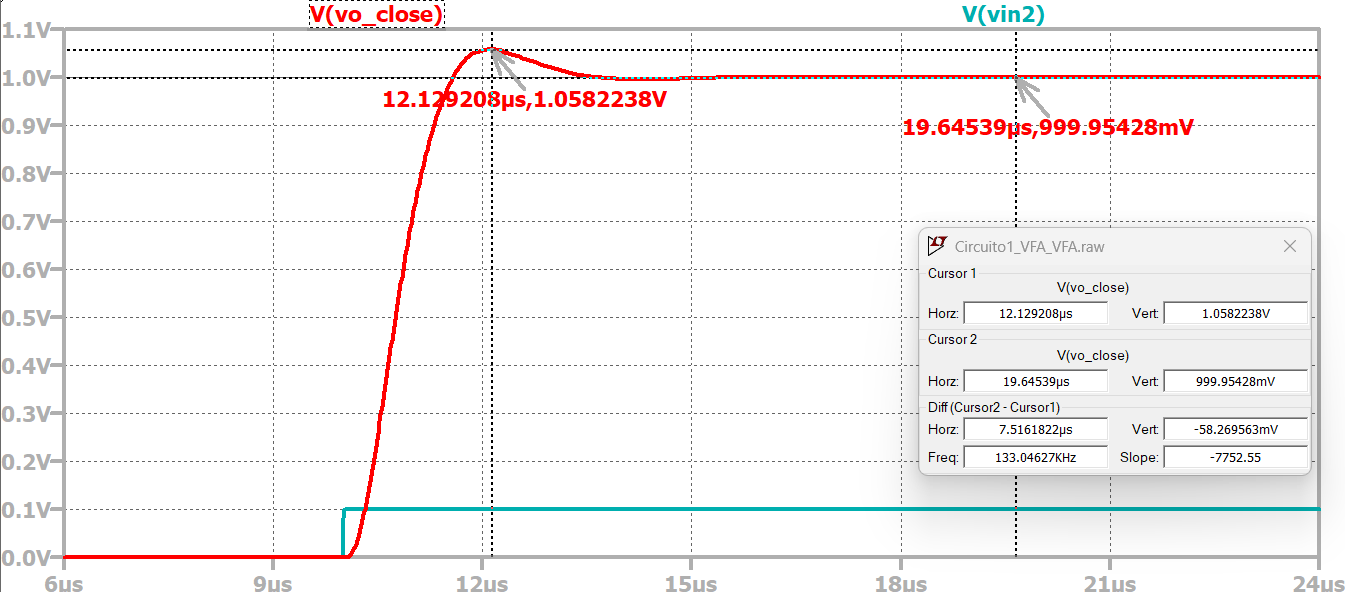
\includegraphics[width=\linewidth,height=0.32\textheight,keepaspectratio]{Imagenes/c1_rta_step.png}
    \caption{Respuesta al escalón de $\SI{0,1}{V}$ (LTSpice): $V_{pico} = \SI{1,0582}{V}$ y $V_{est} = \SI{0,99995}{V}$.}
    \label{fig:rta_step}
\end{figure}

\subsection{Comparación de resultados}
\label{sec:comparacion_c1}

La \autoref{tab:final_c1} compara los valores analíticos (dos polos), el modelo de cuatro polos y las mediciones de LTSpice.

\begin{table}[H]
\centering
\caption{Comparación entre teoría y simulación (VFA-VFA). Error $= (\text{teórico}-\text{LTSpice})/\text{LTSpice}$.}
\label{tab:final_c1}
\small
\setlength{\tabcolsep}{4pt}
\begin{tabularx}{\textwidth}{>{\raggedright\arraybackslash}X c c c c c}
\toprule
\textbf{Magnitud} & \textbf{Analítico} & \textbf{4 polos} & \textbf{LTSpice} & \textbf{Err. anal. [\%]} & \textbf{Err. 4p [\%]} \\
\midrule
Ancho de banda potencial $f_G$ [kHz] & 316,2 & --- & --- & --- & --- \\
Cruce de $T$ asintótico $f_{Gc}$ [kHz] & 223,6 & 206,1 & 206,0 & $+8{,}6$ & $0{,}0$ \\
Cruce de $T$ exacto (2 polos) [kHz] & 203,5 & 206,1 & 206,0 & $-1{,}2$ & $0{,}0$ \\
Margen de fase del lazo [$^\circ$] & 65,53 & 62,51 & 62,52 & $+4{,}8$ & $0{,}0$ \\
Frecuencia de polos $f_p$ [kHz] & 316,2 & 330,3 & --- & --- & --- \\
Ancho de banda real $f_H$ [kHz] & 316,2 & 345,8 & 345,0 & $-8{,}3$ & $+0{,}2$ \\
Sobrepico \%OS [\%] & 4,32 & 5,82 & 5,83 & $-25{,}8$ & $-0{,}1$ \\
$M_\varphi$ desde el escalón [$^\circ$] & 65,53 & 63,57 & 63,56 & $+3{,}1$ & $0{,}0$ \\
\bottomrule
\end{tabularx}
\end{table}

\begin{table}[H]
\centering
\caption{Respuesta al escalón de $0{,}1\text{ V}$ y margen de fase estimado.}
\label{tab:escalon_c1}
\begin{tabular}{lccc}
\toprule
\textbf{Magnitud} & \textbf{2 polos} & \textbf{4 polos} & \textbf{LTSpice} \\
\midrule
$V_{pico}$ [V] & 1,043 & 1,058 & 1,058 \\
$V_{est}$ [V] & 1,000 & 1,000 & 1,000 \\
$\mathrm{\char37}OS$ & 4,32 & 5,82 & 5,83 \\
$\zeta$ & 0,7071 & 0,6711 & 0,6709 \\
$M_\varphi$ estimado [$^\circ$] & 65,53 & 63,57 & 63,56 \\
\bottomrule
\end{tabular}
\end{table}


\subsection{Análisis y conclusión parcial}
\label{sec:concl_c1}

\begin{itemize}
    \item El modelo de dos polos predice un $f_H = f_G = 316{,}2\text{ kHz}$; el modelo de cuatro polos y la simulación dan $\approx 345\text{ kHz}$. La diferencia ($\approx 9\,\mathrm{\char37}$) se debe al segundo polo del LM324 ($f_2$), no incluido en el modelo simple, que eleva ligeramente $Q$ ($0{,}746$) y el ancho de banda.
    \item La frecuencia crítica y el margen de fase medidos en LTSpice ($206{,}0\text{ kHz}$, $62{,}52^\circ$) coinciden con el modelo de cuatro polos (error menor a $0{,}1\,\mathrm{\char37}$), lo que valida el modelo. Respecto del modelo de dos polos el margen de fase es $\approx 3^\circ$ menor, consecuencia del segundo polo.
    \item El margen de fase estimado a partir del escalón ($63{,}6^\circ$) es consistente con el medido en el lazo ($62{,}5^\circ$), con una diferencia de $\approx 1^\circ$; la relación entre sobrepico y margen de fase es aproximada, pues el sistema no es exactamente de segundo orden.
    \item El sobrepico simulado ($5{,}83\,\mathrm{\char37}$) coincide con el del modelo de cuatro polos ($5{,}82\,\mathrm{\char37}$), y es mayor que el del modelo de dos polos ($4{,}32\,\mathrm{\char37}$): el segundo polo del LM324 aumenta el sobrepico. La medición se hizo con un escalón de $0{,}1\text{ V}$ y flancos de $10\text{ ns}$; con un escalón de $1\text{ V}$ (salida de $10\text{ V}$) el sobrepico medido fue menor ($4{,}8\,\mathrm{\char37}$), posiblemente por la limitación de velocidad de respuesta (\emph{slew rate}) del modelo y por el flanco de esa simulación, por lo que no era representativa de pequeña señal.
    \item Se verifica el diseño: ganancia de $20\text{ dB}$, respuesta sin sobrepico en frecuencia y margen de fase cercano a $65^\circ$ (MPM), con un ancho de banda real $\approx 3{,}4$ veces el del amplificador simple ($f_T/A_{vf} = 100\text{ kHz}$).
\end{itemize}
